% !TeX program = lualatex

\documentclass[12pt, a4paper, landscape]{article}

% --- Packages ---
\usepackage{enumitem}
\usepackage{fancyhdr}
\usepackage{fontspec}
\usepackage{geometry}
\usepackage{graphicx}
\usepackage[russian]{babel}
\usepackage{tikz}
\usepackage{titlesec}
\usepackage{hyperref}
\usepackage{xcolor}
\usepackage{wrapfig}

% --- Custom Colors ---
\definecolor{pagebg}{HTML}{F0D7B6}
\definecolor{bordercol}{HTML}{851F23}
\pagecolor{pagebg}

% --- Font ---
\setmainfont[
UprightFont = * Regular,
BoldFont    = * Bold,
ItalicFont  = * Italic,
BoldItalicFont = * BoldItalic,
]{Coats}

% --- Section Title Style ---
\newfontfamily\sectionfont{Coats Bold}\titleformat{\section}
{\sectionfont\fontsize{20pt}{24pt}\selectfont\bfseries\color{bordercol}}
{\thesection}{1em}{}

\titleformat{\subsection}
{\sectionfont\fontsize{15pt}{18pt}\selectfont\bfseries\color{bordercol}}
{\thesection}{1em}{}

% --- Page Border ---
\AddToHook{shipout/foreground}{
    \begin{tikzpicture}[remember picture,overlay]
        \draw[line width=1cm, bordercol]
            (current page.north west) rectangle (current page.south east);
    \end{tikzpicture}
}

% --- Page Setup ---
\geometry{margin=2.5cm}
\pagestyle{fancy}
\fancyhf{}
\fancyfoot[C]{\thepage}
\setlist{itemsep=0pt, topsep=8pt}

\sloppy

\begin{document}

% --- Title ---
\begin{center}
    {\fontspec{Segoe Script}
        \textcolor{bordercol}{\fontsize{36pt}{40pt}\selectfont Легенды Средневековья}
    }
\end{center}

\begin{wrapfigure}{r}{0.32\textwidth}
    \centering
    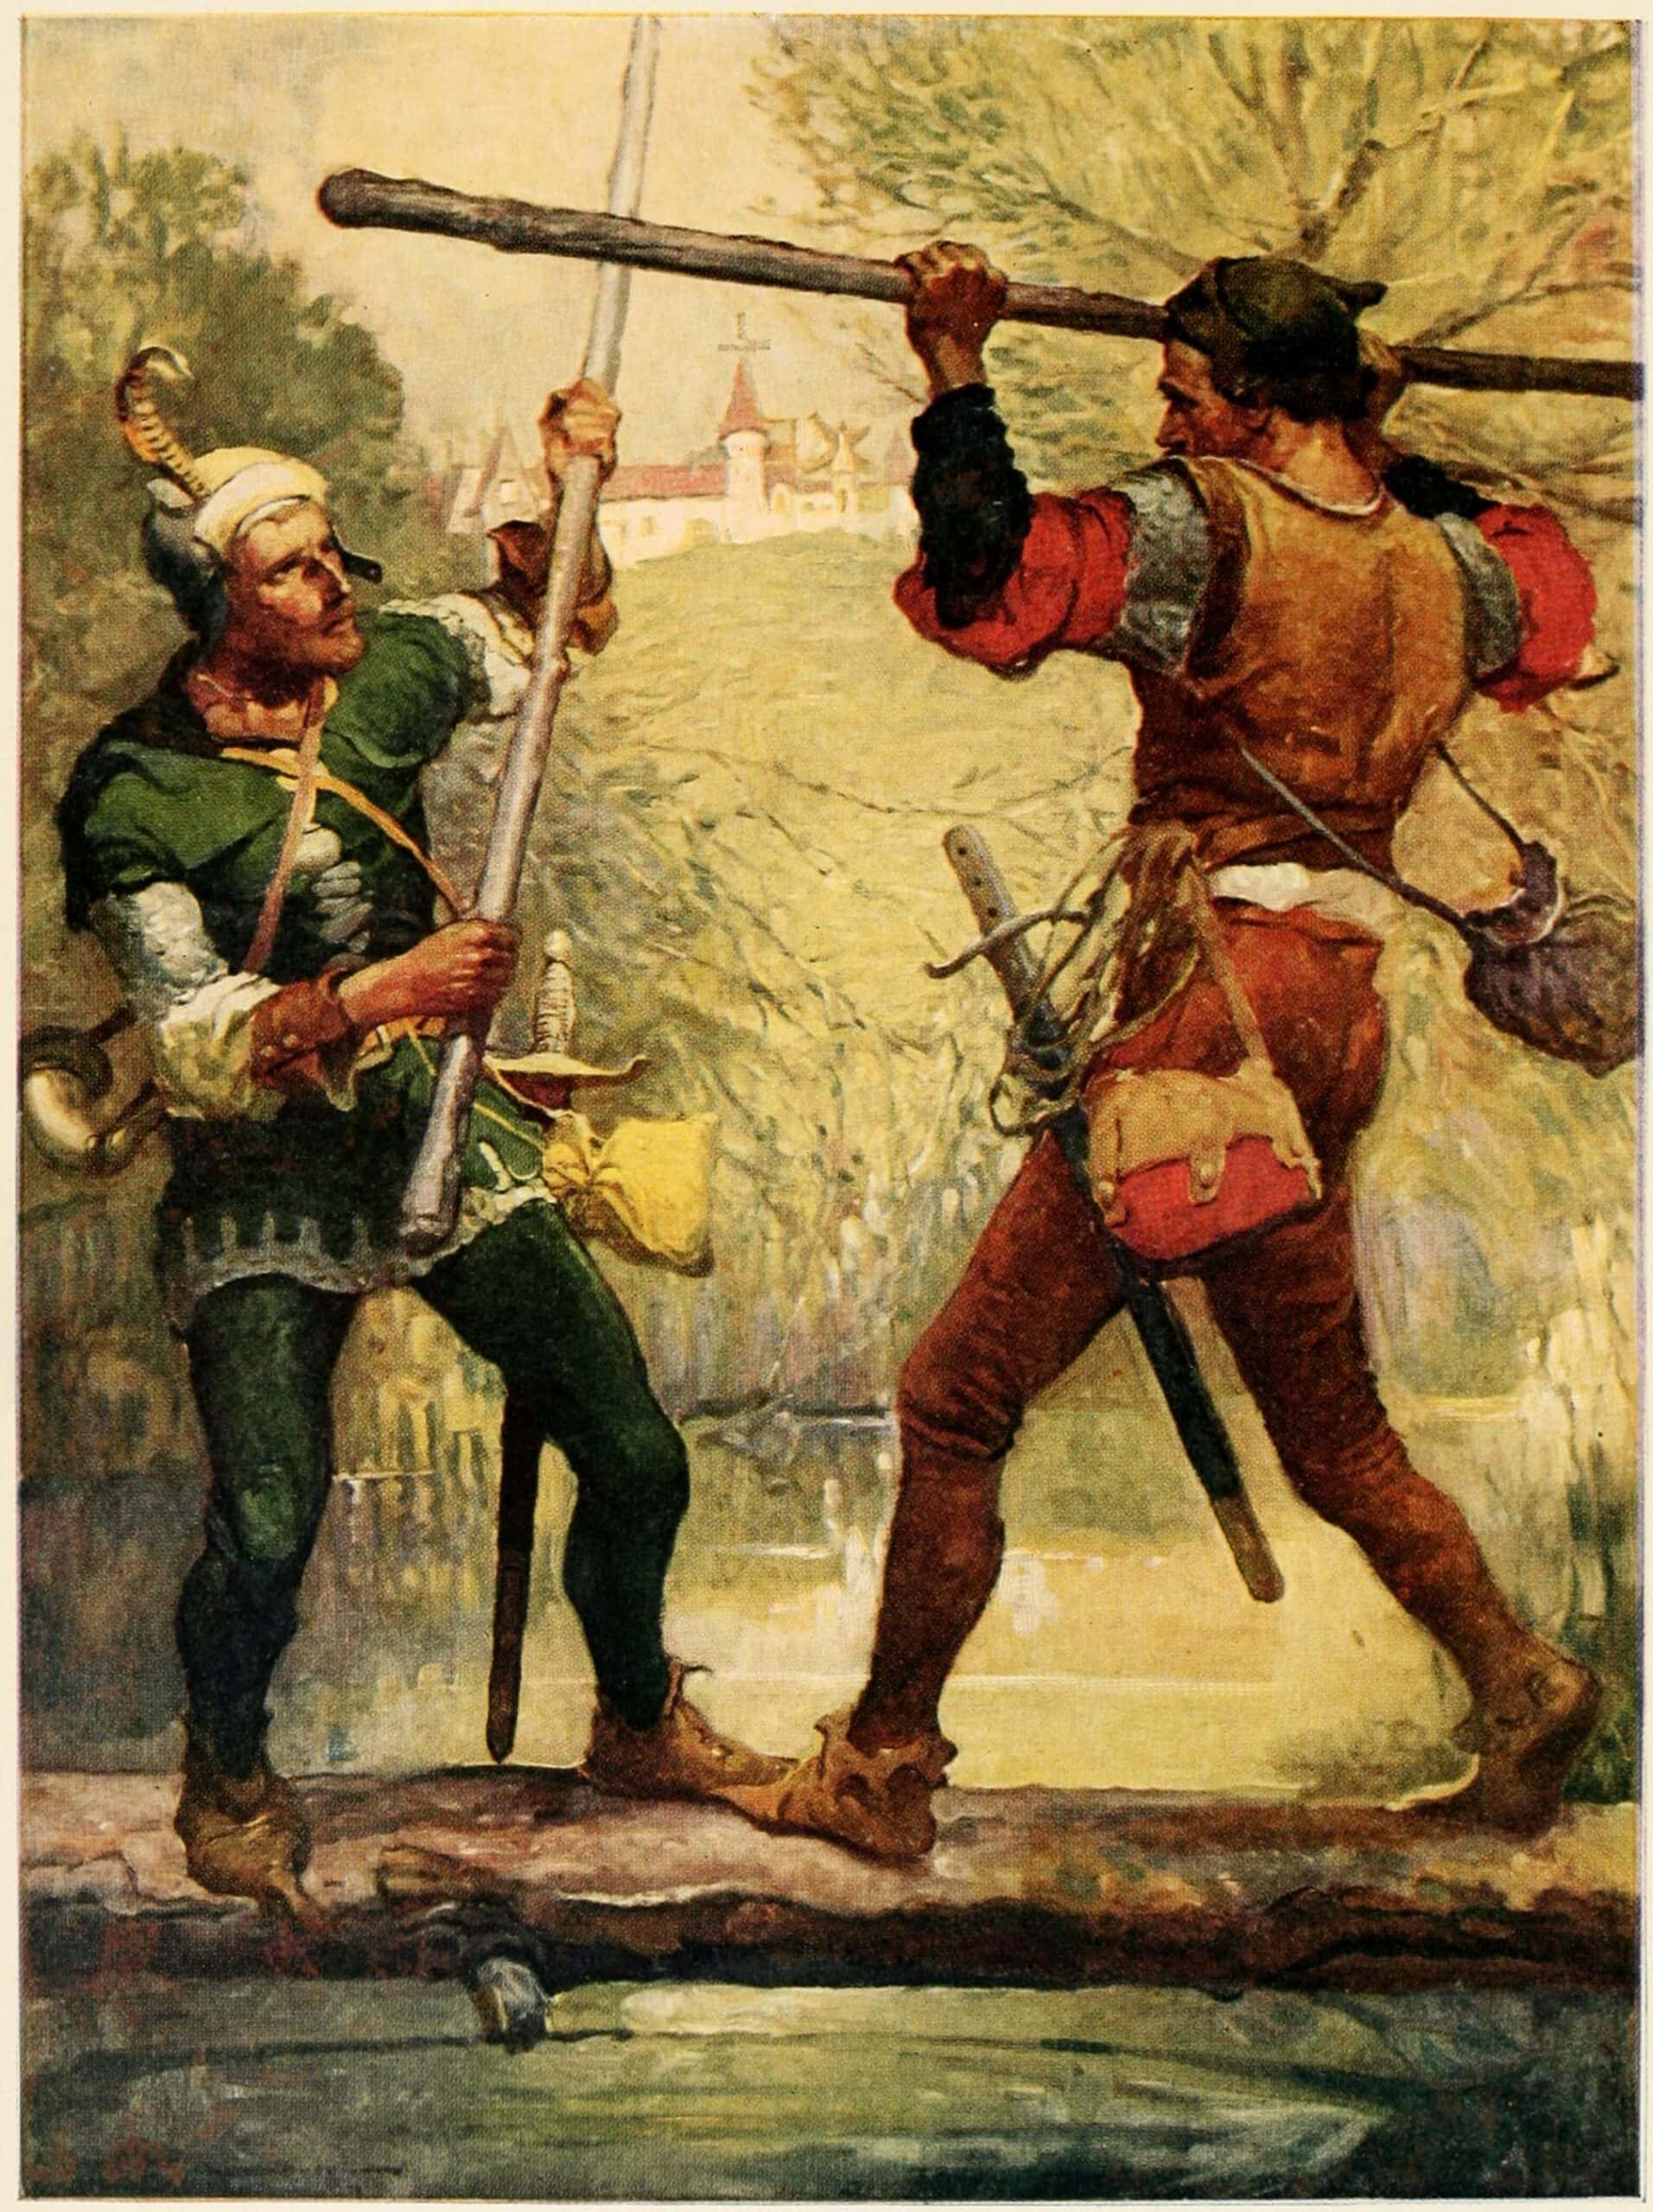
\includegraphics[width=0.30\textwidth]{Robin_Hood_and_Little_John-scaled.jpg}
\end{wrapfigure}

Глубоко в сердце Шервудского леса, среди вековых дубов, королевская
дорога между Лондоном и Йорком подвергалась набегам разбойников.
Богатые были вынуждены отдавать все, что имели, а простые люди
уходили свободными. Нуждающиеся получали одежду, еду и кров. Эта
банда разбойников, грабившая богатых и раздававшая добычу бедным,
противостояла тираническому игу несправедливых лордов и шерифов.
Кто был лидером этих борцов за социальную справедливость?

\textbf{Робин Гуд}, легендарный герой-разбойник из серии английских баллад, некоторые из которых датируются по крайней мере XIV веком. Робин Гуд был мятежником, и многие из самых ярких эпизодов в рассказах о нем показывают, как он и его товарищи грабят и убивают представителей власти, а добычу отдают бедным. Их самым частым врагом был шериф Ноттингема, местный представитель центральной власти (хотя внутренние свидетельства из ранних баллад ясно показывают, что действие происходило главным образом в южном Йоркшире, а не в Ноттингемшире). Среди других врагов были богатые церковные землевладельцы. Робин с уважением относился к женщинам, бедным и людям низкого социального положения. Во многом его восстание против власти было вызвано недовольством народа законами леса, ограничивавшими права на охоту. Ранние баллады, в особенности, раскрывают жестокость, которая была неотъемлемой частью средневековой жизни.

\newpage

\subsection*{Источники}

\begin{itemize}
    \item \href{https://www.nottinghamcastle.org.uk/the-legend-of-robin-hood/}{www.nottinghamcastle.org.uk/the-legend-of-robin-hood/} \\
    \item \href{https://www.historic-uk.com/HistoryUK/HistoryofEngland/Robin-Hood/}{www.historic-uk.com/HistoryUK/HistoryofEngland/Robin-Hood/} \\
    \item \href{https://www.britannica.com/topic/Robin-Hood}{www.britannica.com/topic/Robin-Hood}
\end{itemize}

\end{document}
